\documentclass[12pt,a4paper]{article}

\newcommand{\TETELNUMBER}{21}
\newcommand{\TETELTITLE}{Adatkezelés, adatbázis-architektúra, indexek és normalizálás}
\newcommand{\TETELSHORTTITLE}{Adatkezelés és normalizálás}

\newcommand{\ZVTetelsorDataOnly}{}
\newcommand{\ZVTetelOne}{Adatok, adattípusok, adatműveletek és adatstruktúrák. Szám adattípus. Számrendszerek, konverziók. A logikai, halmaz, karakter, sztring absztrakt adattípusok és realizációjuk. A tömb (vektor, mátrix), rekord absztrakt adattípusok.}
\newcommand{\ZVTetelTwo}{Az algoritmus. Iteratív és rekurzív algoritmus. A számítógépes memória. Adat és program. Verem és procedúra. Az algoritmus lejegyzése. A folyamatábra és a pszeudokód. Elemi algoritmusok.}
\newcommand{\ZVTetelThree}{Strukturált programozás. Programgráf, valódi program, vezérlőgráf lebontása, strukturált program és annak formulája. Strukturált programgráf kialakítása, struktogram. Ciklikus bonyolultság és egyéb bonyolultsági tételek.}
\newcommand{\ZVTetelFour}{Számelméleti algoritmusok. Legnagyobb közös osztó, euklideszi és kibővített euklideszi algoritmus, lineáris kongruencia egyenletek. Multiplikatív inverz, moduláris hatványozás, Fermat prímteszt. RSA.}
\newcommand{\ZVTetelFive}{Rendezések: Beszúró rendezés. Az ,,Oszd meg és uralkodj!'' elv. Összefésülő rendezés. Gyors rendezés. Buborék rendezés. Shell rendezés. Minimum kiválasztásos rendezés. Négyzetes rendezés. Lineáris idejű rendezések: leszámláló rendezés, számjegyes rendezés. Időelemzéseik. Az összehasonlító rendezések időtétele.}
\newcommand{\ZVTetelSix}{Gráfalgoritmusok. Szélességi keresés. Mélységi keresés. Topologikus rendezés. Optimumfeladatok fákon (minimális feszítőfák, Kruskal- és Prim-algoritmus). Legrövidebb utak meghatározása (Dijkstra-algoritmus, Bellman--Ford-algoritmus, Floyd--Warshall-algoritmus).}
\newcommand{\ZVTetelSeven}{A párhuzamos algoritmusok alapfogalmai, PRAM modell, hatékonysági mértékek (munka, költség, gyorsítás, hatékonyság). Párhuzamos végrehajtás ábrázolási módjai. Komplexitás becslése, párhuzamos komplexitás. Amdahl törvénye. Pipeline párhuzamosítás, Lost update probléma bemutatása és megoldása.}
\newcommand{\ZVTetelEight}{Aggregáció, redukció, prefixszámítás párhuzamosítási lehetőségei. \texttt{CREW\_PREFIX}, \texttt{EREW\_PREFIX} és \texttt{OPTIMAL\_PREFIX} algoritmusok bemutatása. Összefésülő rendezés párhuzamosítási módja.}
\newcommand{\ZVTetelNine}{A busz, gyűrű, rács, tórusz, hiperkocka és fa topológiák bemutatása, csomópontok közötti távolságok jellemzése. A CSP, Publish--Subscribe és az Aktor modell. Az aszinkron programozás elemei: async, await kulcsszavak használata, coroutine-ok.}
\newcommand{\ZVTetelTen}{A Turing-gép fogalma, működése. A RAM-gép. Boole-függvények és logikai hálózatok.}
\newcommand{\ZVTetelEleven}{Algoritmikus eldönthetőség. Church-tézis. Rekurzív és rekurzívan felsorolható nyelvek, rekurzív illetve parciálisan rekurzív függvények. Nevezetes nyelvek (Az R, Re, coR, coRE nyelvosztályok és ezek kapcsolata) és bonyolultságuk. Algoritmikusan eldönthetetlen problémák. Polinomiális idejű algoritmusok.}
\newcommand{\ZVTetelTwelve}{Nemdeterminisztikus Turing-gépek, az NP és a coNP nyelvosztály. Példák NP-beli nyelvekre. A tanú-tétel. Nemdeterminisztikus algoritmusok bonyolultsága. NP-teljesség, Cook-tétel. Néhány NP-teljes probléma, Cook--Levin-tétel.}
\newcommand{\ZVTetelThirteen}{A Java programozási nyelv története, alapvető jellemzői. Egy Java program szerkezete (csomagok és fordítási egységek). Az objektumorientált programtervezés alapelveinek felsorolása. Objektumok tárolása és élettartama. Szemétgyűjtő mechanizmus. Kivételkezelés.}
\newcommand{\ZVTetelFourteen}{Az egységbezárás és az információrejtés objektumorientált alapelvek megvalósítása. Osztálydefiníció és példányosítás. Osztályszintű és példányszintű tagok, konstansok. Hozzáférési kategóriák és használatuk. Hivatkozás az osztály tagjaira.}
\newcommand{\ZVTetelFifteen}{Az öröklődés és a polimorfizmus objektumorientált alapelvek megvalósítása. Öröklődés szabályai, metódusok túlterhelése és felüldefiniálása. A referencia statikus és dinamikus típusa. Absztrakt osztály és interfész szerepe, összehasonlítása.}
\newcommand{\ZVTetelSixteen}{Az operációs rendszerbeli folyamat (processz) fogalma. Folyamatkontextus. A fonál (szál) fogalma. A processzállapotok, állapotváltások, processz futási módok. Taszk- és fonálállapotok, állapotátmenetek.}
\newcommand{\ZVTetelSeventeen}{A memóriamenedzselés feladatai. Memória mint erőforrás. Címleképzés fajtái. Lapozós virtuális memóriamenedzselés működése. Allokálás, nyilvántartás, címleképzés. Laphiba fogalma, kezelése, kilapozási stratégiák. Előnyök, hátrányok.}
\newcommand{\ZVTetelEighteen}{Fájlrendszer-megvalósítási feladatok. Jegyzékszerkezetek. Szabadblokk-menedzselési lehetőségek. Fájlattribútum-rögzítési lehetőségek (ezen belül a fájltestet képező blokkok rögzítési lehetőségei).}
\newcommand{\ZVTetelNineteen}{Relációs adatmodell, relációs struktúra és integritási feltételek. ER modell elemei jelentése és jelölése. Az ER modell konverziója relációs modellre. Relációs adatmodell műveleti része, relációs algebra.}
\newcommand{\ZVTetelTwenty}{Az SQL szabvány relációs adatbázis kezelő nyelv bemutatása, a DDL (objektum létrehozás, megszüntetés és szerkezet módosítás), DML (rekord felvitel, törlés és módosítás), DCL és a SELECT utasítások áttekintése és használata. Beágyazott SELECT használata. A relációs algebra műveleteinek megvalósítása SQL-ben.}
\newcommand{\ZVTetelTwentyOne}{Adatkezelés és adatbáziskezelés alapfogalmai, fileszervezési módszerek, B-fa index; adatbázis architektúra; A normalizálás szerepe a relációs adatbázis kezelésben. Redundancia oka és a megszüntetés lépései. Normálformák. Dekompozíció célja és szabályai, tételei.}
\newcommand{\ZVTetelTwentyTwo}{Számítógép-hálózatokhoz kötődő alapfogalmak és az ISO--OSI hivatkozási modell: topológia és méret szerinti osztályozásuk. Kapcsolástechnika szerinti osztályozásuk (vonalkapcsolás, üzenetkapcsolás, csomagkapcsolás és virtuális vonalkapcsolás). Az ISO--OSI hivatkozási modell szerkezete, rétegei és azok főbb funkciói.}
\newcommand{\ZVTetelTwentyThree}{A számítógép-hálózatok ISO--OSI hivatkozási modell adatkapcsolati rétegének közeghozzáférési alrétege: A főbb csatorna-megosztási osztályok (statikus-dinamikus, dinamikus versengő-determinisztikus) bemutatása és azok összevetése. Az IEEE 802.3 és az Ethernet (CSMA/CD) keretformátum, MAC címek, támogatott közegek és sebességek bemutatása, működés duplex csatorna esetén. Az IEEE 802.11 WLAN általános felépítése, az Access Point (AP) főbb funkciói. Az alkalmazott közeghozzáférési módszer (CSMA/CA), Distributed Coordination Function (DCF) és Point Coordination Function (PCF) üzemmódok.}
\newcommand{\ZVTetelTwentyFour}{A TCP/IP protokollszövet és az Internet. Az Internet hivatkozási modell (DoD) és az ISO--OSI hivatkozási modell összevetése. A TCP/IP protokollszövet főbb részei (ARP, RARP, IP, ICMP, TCP, UDP) és azok funkciói. Az internetes címzés és címosztályok: IPv4-címosztályok, maszk, subnet, supernet, osztály nélküli címzés (CIDR -- Classless Inter-Domain Routing) és változó alhálózat-méretek (VLSM -- Variable Length Subnet Mask), címek kiosztása, lokális címek és címfordítás (NAT). IPv6-címek, IPv6-címtípusok (unicast, multicast, anycast; link local, unique local, aggregatable global unicast address).}
\newcommand{\ZVTetelTwentyFive}{Szoftvertechnológia és a szoftverfolyamat fogalma. A szoftverfolyamat-fázisok részletes bemutatása: szoftverspecifikáció, tervezés, implementáció, validáció és evolúció. Az evolúciós modell ismertetése.}
\newcommand{\ZVTetelTwentySix}{Szoftverkövetelmény fogalma és osztályozásai. Követelmények általános problémái. Követelményfeltárás és -elemzés folyamata. Vezérlési stílusok.}
\newcommand{\ZVTetelTwentySeven}{UML diagramok bemutatása: Use case és osztálydiagram. A szekvenciadiagram. Komponensdiagram.}

\newcommand{\ZVTetelKiiras}[1]{%
  \ifcase#1\relax
  \or \ZVTetelOne
  \or \ZVTetelTwo
  \or \ZVTetelThree
  \or \ZVTetelFour
  \or \ZVTetelFive
  \or \ZVTetelSix
  \or \ZVTetelSeven
  \or \ZVTetelEight
  \or \ZVTetelNine
  \or \ZVTetelTen
  \or \ZVTetelEleven
  \or \ZVTetelTwelve
  \or \ZVTetelThirteen
  \or \ZVTetelFourteen
  \or \ZVTetelFifteen
  \or \ZVTetelSixteen
  \or \ZVTetelSeventeen
  \or \ZVTetelEighteen
  \or \ZVTetelNineteen
  \or \ZVTetelTwenty
  \or \ZVTetelTwentyOne
  \or \ZVTetelTwentyTwo
  \or \ZVTetelTwentyThree
  \or \ZVTetelTwentyFour
  \or \ZVTetelTwentyFive
  \or \ZVTetelTwentySix
  \or \ZVTetelTwentySeven
  \fi
}

\newcommand{\ZVTetelsorList}{%
\begin{enumerate}[leftmargin=7mm,label=\arabic*.,itemsep=2pt,topsep=2pt,parsep=0pt]
  \item \ZVTetelOne
  \item \ZVTetelTwo
  \item \ZVTetelThree
  \item \ZVTetelFour
  \item \ZVTetelFive
  \item \ZVTetelSix
  \item \ZVTetelSeven
  \item \ZVTetelEight
  \item \ZVTetelNine
  \item \ZVTetelTen
  \item \ZVTetelEleven
  \item \ZVTetelTwelve
  \item \ZVTetelThirteen
  \item \ZVTetelFourteen
  \item \ZVTetelFifteen
  \item \ZVTetelSixteen
  \item \ZVTetelSeventeen
  \item \ZVTetelEighteen
  \item \ZVTetelNineteen
  \item \ZVTetelTwenty
  \item \ZVTetelTwentyOne
  \item \ZVTetelTwentyTwo
  \item \ZVTetelTwentyThree
  \item \ZVTetelTwentyFour
  \item \ZVTetelTwentyFive
  \item \ZVTetelTwentySix
  \item \ZVTetelTwentySeven
\end{enumerate}%
}


\newcommand{\tetelsorrow}[2]{\textbf{#1.} & #2\tabularnewline}

\newcommand{\tetelsorpageone}{%
\begin{tabularx}{\textwidth}{|>{\raggedleft\bfseries}p{8mm}@{\hspace{5mm}}>{\raggedright\arraybackslash}X|}
\hline
\tetelsorrow{1}{\ZVTetelOne}
\tetelsorrow{2}{\ZVTetelTwo}
\tetelsorrow{3}{\ZVTetelThree}
\hline
\tetelsorrow{4}{\ZVTetelFour}
\tetelsorrow{5}{\ZVTetelFive}
\tetelsorrow{6}{\ZVTetelSix}
\hline
\tetelsorrow{7}{\ZVTetelSeven}
\tetelsorrow{8}{\ZVTetelEight}
\tetelsorrow{9}{\ZVTetelNine}
\hline
\tetelsorrow{10}{\ZVTetelTen}
\tetelsorrow{11}{\ZVTetelEleven}
\tetelsorrow{12}{\ZVTetelTwelve}
\hline
\end{tabularx}%
}

\newcommand{\tetelsorpagetwo}{%
\begin{tabularx}{\textwidth}{|>{\raggedleft\bfseries}p{8mm}@{\hspace{5mm}}>{\raggedright\arraybackslash}X|}
\hline
\tetelsorrow{13}{\ZVTetelThirteen}
\tetelsorrow{14}{\ZVTetelFourteen}
\tetelsorrow{15}{\ZVTetelFifteen}
\hline
\tetelsorrow{16}{\ZVTetelSixteen}
\tetelsorrow{17}{\ZVTetelSeventeen}
\tetelsorrow{18}{\ZVTetelEighteen}
\hline
\tetelsorrow{19}{\ZVTetelNineteen}
\tetelsorrow{20}{\ZVTetelTwenty}
\tetelsorrow{21}{\ZVTetelTwentyOne}
\hline
\tetelsorrow{22}{\ZVTetelTwentyTwo}
\tetelsorrow{23}{\ZVTetelTwentyThree}
\tetelsorrow{24}{\ZVTetelTwentyFour}
\hline
\tetelsorrow{25}{\ZVTetelTwentyFive}
\tetelsorrow{26}{\ZVTetelTwentySix}
\tetelsorrow{27}{\ZVTetelTwentySeven}
\hline
\end{tabularx}%
}

\ifdefined\ZVTetelsorDataOnly
\expandafter\endinput
\fi

\documentclass[10pt,a4paper]{article}
\newcommand{\ZVHEADERLEFT}{Záróvizsga tételek}
\newcommand{\ZVHEADERRIGHT}{Programtervező informatikus BSc}
\usepackage{fontspec}
\usepackage{geometry}
\usepackage{microtype}
\usepackage{xcolor}
\usepackage{amsmath,amssymb,mathtools}
\usepackage{booktabs,longtable,tabularx,array,multirow}
\usepackage{enumitem}
\usepackage{hyperref}
\usepackage{fancyhdr}
\usepackage{titlesec}
\usepackage{listings}
\usepackage[most]{tcolorbox}
\usepackage{tikz}
\usetikzlibrary{positioning,shapes.geometric,shapes.misc,arrows.meta,decorations.pathreplacing}
\usepackage{caption}

\setlength{\headheight}{16pt}
\emergencystretch=2em
\renewcommand{\contentsname}{Tartalom}

% Fontbeallitasok: ha a DejaVu fontok nincsenek telepitve,
% akkor automatikusan a MiKTeX/TeX Live alap Latin Modern fontjaira valtunk.
\IfFontExistsTF{DejaVu Serif}{\setmainfont{DejaVu Serif}}{\setmainfont{Latin Modern Roman}}
\IfFontExistsTF{DejaVu Sans}{\setsansfont{DejaVu Sans}}{\setsansfont{Latin Modern Sans}}
\IfFontExistsTF{DejaVu Sans Mono}{\setmonofont{DejaVu Sans Mono}}{\setmonofont{Latin Modern Mono}}

\geometry{left=25mm,right=25mm,top=24mm,bottom=27mm}

\hypersetup{
  colorlinks=true,
  linkcolor=blue!45!black,
  urlcolor=blue!55!black,
  pdftitle={Zarovizsga tetel},
  pdfauthor={Baba Levente - tanulasi segedanyag}
}

\definecolor{accent}{HTML}{1F4E79}
\definecolor{lightaccent}{HTML}{EAF2F8}
\definecolor{warnbg}{HTML}{FFF4E5}
\definecolor{codebg}{HTML}{F7F7F7}

\tikzset{
  flow/.style={draw, rounded corners, align=center, minimum width=21mm, minimum height=8mm, fill=lightaccent},
  pred/.style={draw, diamond, aspect=2, align=center, inner sep=1pt, fill=warnbg},
  merge/.style={draw, circle, inner sep=1.2pt, fill=black!8},
  terminator/.style={draw, rounded corners=4mm, align=center, minimum width=20mm, minimum height=8mm, fill=black!5},
  arrow/.style={->, >=stealth, thick},
  zvflowstart/.style={draw, rounded rectangle, minimum width=2.3cm, minimum height=0.7cm, align=center},
  zvflowprocess/.style={draw, rectangle, minimum width=2.7cm, minimum height=0.7cm, align=center},
  zvflowdecision/.style={draw, diamond, aspect=2.2, minimum width=2.8cm, minimum height=0.8cm, align=center}
}


\titleformat{\section}{\Large\bfseries\sffamily\color{accent}}{\thesection.}{0.6em}{}
\titleformat{\subsection}{\large\bfseries\sffamily\color{accent}}{\thesubsection.}{0.6em}{}
\titleformat{\subsubsection}{\normalsize\bfseries\sffamily\color{accent}}{\thesubsubsection.}{0.6em}{}

\setlist[itemize]{topsep=3pt,itemsep=2pt,parsep=0pt,leftmargin=1.4em}
\setlist[enumerate]{topsep=3pt,itemsep=2pt,parsep=0pt,leftmargin=1.6em}
\setlength{\parindent}{0pt}
\setlength{\parskip}{6pt}
\renewcommand{\arraystretch}{1.25}
\newcolumntype{L}[1]{>{\raggedright\arraybackslash}p{#1}}
\renewcommand{\tabularxcolumn}[1]{>{\raggedright\arraybackslash}p{#1}}

\providecommand{\ZVHEADERLEFT}{\TETELNUMBER. tétel}
\providecommand{\ZVHEADERRIGHT}{\TETELSHORTTITLE}

\pagestyle{fancy}
\fancyhf{}
\lhead{\ZVHEADERLEFT}
\rhead{\ZVHEADERRIGHT}
\cfoot{\thepage}

\lstdefinelanguage{pseudocode}{
  morekeywords={IF,THEN,ELSE,WHILE,DO,FOR,TO,DOWNTO,REPEAT,UNTIL,RETURN,CALL,INPUT,OUTPUT,AND,OR,NOT,TRUE,FALSE},
  sensitive=true,
  morecomment=[l]{//}
}

\lstdefinestyle{code}{
  basicstyle=\ttfamily\small,
  backgroundcolor=\color{codebg},
  frame=single,
  rulecolor=\color{black!15},
  columns=fullflexible,
  keepspaces=true,
  breaklines=true,
  tabsize=2,
  showstringspaces=false,
  numbers=left,
  numberstyle=\tiny\color{black!55},
  numbersep=7pt,
  xleftmargin=2.2em,
  framexleftmargin=1.7em,
  captionpos=b
}

\lstdefinestyle{pseudo}{
  style=code,
  language=pseudocode,
  keywordstyle=\bfseries\color{accent!85!black},
  commentstyle=\itshape\color{black!55}
}

\lstdefinestyle{csource}{
  style=code,
  language=C,
  keywordstyle=\bfseries\color{accent!85!black},
  commentstyle=\itshape\color{black!55},
  stringstyle=\color{orange!70!black}
}

\lstset{style=code}
\renewcommand{\lstlistingname}{Kódrészlet}
\renewcommand{\lstlistlistingname}{Kódrészletek}
\newcommand{\zvcode}[2][]{\lstinputlisting[style=code,#1]{#2}}
\newcommand{\zvpseudocode}[2][]{\lstinputlisting[style=pseudo,#1]{#2}}
\newcommand{\zvccode}[2][]{\lstinputlisting[style=csource,#1]{#2}}

\newtcolorbox{summarybox}{
  enhanced,
  colback=lightaccent,
  colframe=accent!70!black,
  arc=2mm,
  boxrule=0.5pt,
  left=2mm,right=2mm,top=1mm,bottom=1mm
}

\newtcolorbox{warningbox}{
  enhanced,
  colback=warnbg,
  colframe=orange!70!black,
  arc=2mm,
  boxrule=0.5pt,
  left=2mm,right=2mm,top=1mm,bottom=1mm
}

\newcommand{\adt}[2]{\ensuremath{#1=(#2)}}
\newcommand{\set}[1]{\ensuremath{\{#1\}}}
\newcommand{\code}[1]{\texttt{#1}}
\newcommand{\base}[2]{\ensuremath{#1_{(#2)}}}
\newcommand{\addr}{\ensuremath{@}}


\providecommand{\TETELKIIRAS}{\TETELTITLE. \TETELTOPIC}
\providecommand{\ZVAUTHOR}{Baba Levente}
\providecommand{\ZVYEAR}{2026}
\providecommand{\ZVAID}{ChatGPT segítségével}

\newcommand{\makezvtitle}{%
\begin{titlepage}
  \centering
  \vspace*{18mm}
  {\Large\sffamily Programtervező Informatikus BSc\par}
  \vspace{1mm}
  {\large\sffamily \ZVYEAR-os záróvizsga tételek\par}
  \vspace{15mm}
  {\Huge\bfseries\sffamily \TETELNUMBER. tétel\par}
  \vspace{5mm}
  {\LARGE\bfseries\sffamily \TETELTITLE\par}
  \vspace{10mm}
  \begin{summarybox}
    \textbf{Tételkiírás:} \TETELKIIRAS
  \end{summarybox}
  \vfill
  {\large Készítette: \textbf{\ZVAUTHOR}\par}
  \vspace{2mm}
  {\large \ZVAID\par}
\end{titlepage}%
}

\newcommand{\zvfrontmatter}{%
  \sloppy
  \makezvtitle
  \tableofcontents
  \newpage
}

\begin{document}
\newgeometry{left=13mm,right=13mm,top=13mm,bottom=13mm}
\pagestyle{empty}
\setlength{\tabcolsep}{2.6pt}
\renewcommand{\arraystretch}{1.08}
\begin{center}
  {\Huge\bfseries Záróvizsga tételek\par}
  \vspace{2mm}
  {\Large\itshape Programtervező informatikus BSc\par}
\end{center}
\vspace{10mm}
{\fontsize{10.5}{12.2}\selectfont
\tetelsorpageone
}
\newpage
{\fontsize{10.5}{12.2}\selectfont
\tetelsorpagetwo
}
\end{document}

\newcommand{\TETELKIIRAS}{\ZVTetelKiiras{\TETELNUMBER}}

\usepackage{fontspec}
\usepackage{geometry}
\usepackage{microtype}
\usepackage{xcolor}
\usepackage{amsmath,amssymb,mathtools}
\usepackage{booktabs,longtable,tabularx,array,multirow}
\usepackage{enumitem}
\usepackage{hyperref}
\usepackage{fancyhdr}
\usepackage{titlesec}
\usepackage{listings}
\usepackage[most]{tcolorbox}
\usepackage{tikz}
\usetikzlibrary{positioning,shapes.geometric,shapes.misc,arrows.meta,decorations.pathreplacing}
\usepackage{caption}

\setlength{\headheight}{16pt}
\emergencystretch=2em
\renewcommand{\contentsname}{Tartalom}

% Fontbeallitasok: ha a DejaVu fontok nincsenek telepitve,
% akkor automatikusan a MiKTeX/TeX Live alap Latin Modern fontjaira valtunk.
\IfFontExistsTF{DejaVu Serif}{\setmainfont{DejaVu Serif}}{\setmainfont{Latin Modern Roman}}
\IfFontExistsTF{DejaVu Sans}{\setsansfont{DejaVu Sans}}{\setsansfont{Latin Modern Sans}}
\IfFontExistsTF{DejaVu Sans Mono}{\setmonofont{DejaVu Sans Mono}}{\setmonofont{Latin Modern Mono}}

\geometry{left=25mm,right=25mm,top=24mm,bottom=27mm}

\hypersetup{
  colorlinks=true,
  linkcolor=blue!45!black,
  urlcolor=blue!55!black,
  pdftitle={Zarovizsga tetel},
  pdfauthor={Baba Levente - tanulasi segedanyag}
}

\definecolor{accent}{HTML}{1F4E79}
\definecolor{lightaccent}{HTML}{EAF2F8}
\definecolor{warnbg}{HTML}{FFF4E5}
\definecolor{codebg}{HTML}{F7F7F7}

\tikzset{
  flow/.style={draw, rounded corners, align=center, minimum width=21mm, minimum height=8mm, fill=lightaccent},
  pred/.style={draw, diamond, aspect=2, align=center, inner sep=1pt, fill=warnbg},
  merge/.style={draw, circle, inner sep=1.2pt, fill=black!8},
  terminator/.style={draw, rounded corners=4mm, align=center, minimum width=20mm, minimum height=8mm, fill=black!5},
  arrow/.style={->, >=stealth, thick},
  zvflowstart/.style={draw, rounded rectangle, minimum width=2.3cm, minimum height=0.7cm, align=center},
  zvflowprocess/.style={draw, rectangle, minimum width=2.7cm, minimum height=0.7cm, align=center},
  zvflowdecision/.style={draw, diamond, aspect=2.2, minimum width=2.8cm, minimum height=0.8cm, align=center}
}


\titleformat{\section}{\Large\bfseries\sffamily\color{accent}}{\thesection.}{0.6em}{}
\titleformat{\subsection}{\large\bfseries\sffamily\color{accent}}{\thesubsection.}{0.6em}{}
\titleformat{\subsubsection}{\normalsize\bfseries\sffamily\color{accent}}{\thesubsubsection.}{0.6em}{}

\setlist[itemize]{topsep=3pt,itemsep=2pt,parsep=0pt,leftmargin=1.4em}
\setlist[enumerate]{topsep=3pt,itemsep=2pt,parsep=0pt,leftmargin=1.6em}
\setlength{\parindent}{0pt}
\setlength{\parskip}{6pt}
\renewcommand{\arraystretch}{1.25}
\newcolumntype{L}[1]{>{\raggedright\arraybackslash}p{#1}}
\renewcommand{\tabularxcolumn}[1]{>{\raggedright\arraybackslash}p{#1}}

\providecommand{\ZVHEADERLEFT}{\TETELNUMBER. tétel}
\providecommand{\ZVHEADERRIGHT}{\TETELSHORTTITLE}

\pagestyle{fancy}
\fancyhf{}
\lhead{\ZVHEADERLEFT}
\rhead{\ZVHEADERRIGHT}
\cfoot{\thepage}

\lstdefinelanguage{pseudocode}{
  morekeywords={IF,THEN,ELSE,WHILE,DO,FOR,TO,DOWNTO,REPEAT,UNTIL,RETURN,CALL,INPUT,OUTPUT,AND,OR,NOT,TRUE,FALSE},
  sensitive=true,
  morecomment=[l]{//}
}

\lstdefinestyle{code}{
  basicstyle=\ttfamily\small,
  backgroundcolor=\color{codebg},
  frame=single,
  rulecolor=\color{black!15},
  columns=fullflexible,
  keepspaces=true,
  breaklines=true,
  tabsize=2,
  showstringspaces=false,
  numbers=left,
  numberstyle=\tiny\color{black!55},
  numbersep=7pt,
  xleftmargin=2.2em,
  framexleftmargin=1.7em,
  captionpos=b
}

\lstdefinestyle{pseudo}{
  style=code,
  language=pseudocode,
  keywordstyle=\bfseries\color{accent!85!black},
  commentstyle=\itshape\color{black!55}
}

\lstdefinestyle{csource}{
  style=code,
  language=C,
  keywordstyle=\bfseries\color{accent!85!black},
  commentstyle=\itshape\color{black!55},
  stringstyle=\color{orange!70!black}
}

\lstset{style=code}
\renewcommand{\lstlistingname}{Kódrészlet}
\renewcommand{\lstlistlistingname}{Kódrészletek}
\newcommand{\zvcode}[2][]{\lstinputlisting[style=code,#1]{#2}}
\newcommand{\zvpseudocode}[2][]{\lstinputlisting[style=pseudo,#1]{#2}}
\newcommand{\zvccode}[2][]{\lstinputlisting[style=csource,#1]{#2}}

\newtcolorbox{summarybox}{
  enhanced,
  colback=lightaccent,
  colframe=accent!70!black,
  arc=2mm,
  boxrule=0.5pt,
  left=2mm,right=2mm,top=1mm,bottom=1mm
}

\newtcolorbox{warningbox}{
  enhanced,
  colback=warnbg,
  colframe=orange!70!black,
  arc=2mm,
  boxrule=0.5pt,
  left=2mm,right=2mm,top=1mm,bottom=1mm
}

\newcommand{\adt}[2]{\ensuremath{#1=(#2)}}
\newcommand{\set}[1]{\ensuremath{\{#1\}}}
\newcommand{\code}[1]{\texttt{#1}}
\newcommand{\base}[2]{\ensuremath{#1_{(#2)}}}
\newcommand{\addr}{\ensuremath{@}}


\providecommand{\TETELKIIRAS}{\TETELTITLE. \TETELTOPIC}
\providecommand{\ZVAUTHOR}{Baba Levente}
\providecommand{\ZVYEAR}{2026}
\providecommand{\ZVAID}{ChatGPT segítségével}

\newcommand{\makezvtitle}{%
\begin{titlepage}
  \centering
  \vspace*{18mm}
  {\Large\sffamily Programtervező Informatikus BSc\par}
  \vspace{1mm}
  {\large\sffamily \ZVYEAR-os záróvizsga tételek\par}
  \vspace{15mm}
  {\Huge\bfseries\sffamily \TETELNUMBER. tétel\par}
  \vspace{5mm}
  {\LARGE\bfseries\sffamily \TETELTITLE\par}
  \vspace{10mm}
  \begin{summarybox}
    \textbf{Tételkiírás:} \TETELKIIRAS
  \end{summarybox}
  \vfill
  {\large Készítette: \textbf{\ZVAUTHOR}\par}
  \vspace{2mm}
  {\large \ZVAID\par}
\end{titlepage}%
}

\newcommand{\zvfrontmatter}{%
  \sloppy
  \makezvtitle
  \tableofcontents
  \newpage
}


\begin{document}
\zvfrontmatter
\section{A tétel lényege és vizsgaszintű vázlata}

\begin{summarybox}
A 21. tétel az adatbázis-kezelés gyakorlati hátterét és a relációs sémák helyes kialakítását foglalja össze. Először az adatkezelés, adatbázis, DBMS, metaadat és adatmodell alapfogalmait kell tisztázni. Ezután érdemes bemutatni, hogy a fájlalapú adatkezelés milyen korlátokba ütközik, milyen fájlszervezési módszerek léteznek, és ezekhez képest mit ad egy adatbázis-kezelő rendszer. A tétel második nagy része az indexelés, különösen a B-fa index, majd a normalizálás: redundancia, anomáliák, funkcionális függőségek, normálformák és dekompozíciós szabályok.
\end{summarybox}

Vizsgán célszerű a következő sorrendet követni:

\begin{enumerate}
  \item adatkezelés, adatbázis, DBMS, adatmodell és metaadat fogalma;
  \item fájlalapú adatkezelés előnyei és korlátai;
  \item fájlszervezési módszerek: heap, szekvenciális, index-szekvenciális, indexelt, hash, klaszterezett és particionált;
  \item adatbázis-architektúra és a DBMS rétegei;
  \item index fogalma, szerepe, előnyei és költségei;
  \item B-fa/B\textsuperscript{+}-fa index felépítése és műveletei;
  \item redundancia, adatbázis-anomáliák és funkcionális függőségek;
  \item 1NF, 2NF, 3NF, BCNF, röviden 4NF;
  \item dekompozíció célja, veszteségmentesség, függőségmegőrzés, Heath- és Rissanen-tétel;
  \item gyakori vizsgahibák és rövid összefoglaló válasz.
\end{enumerate}

A legfontosabb vizsgamondat: az adatbázis-kezelő rendszer a fájlalapú adatkezelés fölé épülő általános szerverkomponens, amely sémával, metaadatokkal, indexekkel, jogosultságokkal, tranzakciókezeléssel és optimalizálással biztosítja az adatok hatékony és biztonságos kezelését; a normalizálás pedig a redundanciát okozó függőségek megszüntetésére szolgáló sémaátalakítási folyamat.

\section{Adatkezelés és adatbáziskezelés alapfogalmai}

\subsection{Adat, információ, adatkezelés}

Az \textbf{adat} valamilyen tény, mérési eredmény, leíró érték vagy jel, amely önmagában még nem feltétlenül hordoz teljes jelentést. Az \textbf{információ} értelmezett adat: olyan adat, amely egy adott felhasználó vagy rendszer számára jelentéssel bír, és döntést vagy műveletet támogat.

Az \textbf{adatkezelés} az adatok létrehozásával, tárolásával, visszakeresésével, módosításával, törlésével, védelmével és továbbításával kapcsolatos műveletek összessége. Egy egyszerű programban ez lehet fájlba írás és fájlból olvasás. Nagyobb információs rendszerben már szükség van hatékony keresésre, többfelhasználós működésre, adatvédelemre, konkurenciakezelésre, integritásra és helyreállíthatóságra is.

A szokásos CRUD műveletek:

\begin{itemize}
  \item \textbf{Create}: új adat létrehozása vagy beszúrása;
  \item \textbf{Read}: adatok lekérdezése, olvasása;
  \item \textbf{Update}: meglévő adatok módosítása;
  \item \textbf{Delete}: adatok törlése.
\end{itemize}

A fájlalapú adatkezelésnél ezeket a műveleteket közvetlenül az alkalmazásprogram valósítja meg. Adatbázis-kezelésnél a műveleteket egy általános adatbázis-kezelő rendszer végzi, amely a felhasználói parancsokat, például SQL utasításokat, belső tárolási műveletekre fordítja.

\subsection{Adatbázis és DBMS}

Az \textbf{adatbázis} logikailag összetartozó, tartósan tárolt adatok és metaadatok rendszere. Nem csak rekordok halmaza, hanem tartalmazhatja az adatok szerkezetét, kapcsolatait, megkötéseit, jogosultsági leírásait és a hatékony elérést segítő objektumokat is.

A \textbf{DBMS} (Database Management System), vagyis adatbázis-kezelő rendszer olyan szoftverrendszer, amely szabályozott módon biztosítja az adatok tárolását, lekérdezését, módosítását, védelmét és helyreállítását. A DBMS feladata, hogy az alkalmazásoknak magasabb szintű, adatmodell szerinti felületet adjon, miközben elrejti a fizikai tárolás sok részletét.

Fontos DBMS-feladatok:

\begin{itemize}
  \item adatdefiníció és séma kezelése;
  \item lekérdezések feldolgozása és optimalizálása;
  \item rekordok tárolása, indexek és fájlok kezelése;
  \item integritási feltételek ellenőrzése;
  \item jogosultságkezelés és adatvédelem;
  \item tranzakciókezelés, konkurenciakezelés, naplózás és helyreállítás;
  \item metaadatok és statisztikák nyilvántartása.
\end{itemize}

A \textbf{metaadat} adat az adatról. Ilyen például egy tábla neve, mezőinek neve és típusa, az elsődleges kulcs, az idegen kulcs, egy index definíciója, egy jogosultsági bejegyzés vagy az optimalizáló által használt statisztika.

\subsection{Adatmodell szerepe}

Az \textbf{adatmodell} meghatározza, hogy az adatok milyen szerkezetben jelenhetnek meg, milyen megkötések érvényesek rájuk, és milyen műveletek végezhetők rajtuk. Három fő része van:

\begin{itemize}
  \item \textbf{szerkezeti rész}: hogyan épül fel az adatbázis, például relációkból, dokumentumokból, gráfcsomópontokból;
  \item \textbf{integritási rész}: milyen értékek és kapcsolatok tekinthetők helyesnek;
  \item \textbf{műveleti rész}: milyen műveletekkel kérdezhetők le és módosíthatók az adatok.
\end{itemize}

A relációs adatmodellben az adatok relációkban, vagyis táblákhoz hasonló logikai szerkezetekben jelennek meg. A kapcsolatok idegen kulcsokkal, az adatok helyessége integritási feltételekkel, a lekérdezések pedig relációs algebrai elveken alapuló SQL utasításokkal kezelhetők.

\begin{center}
\begin{tabularx}{\textwidth}{L{31mm}L{38mm}X}
\toprule
\textbf{Szempont} & \textbf{Fájlalapú adatkezelés} & \textbf{Adatbázis-kezelés DBMS-sel} \\
\midrule
Adatok szerkezete & Az alkalmazás kódja ismeri a fájl formátumát, rekordhosszát és kapcsolatait. & A szerkezet metaadatként, sémában és katalógusban jelenik meg. \\
Kapcsolatok kezelése & Kézzel, programlogikával, sokszor ismétléssel vagy külön fájlokkal. & Kulcsokkal, idegen kulcsokkal, integritási feltételekkel és lekérdezésekkel. \\
Keresés & Szekvenciális feldolgozás vagy kézzel épített index. & Optimalizált végrehajtás, indexek, B-fa vagy hash alapú elérés. \\
Konkurencia & Az alkalmazásnak kell kezelnie a párhuzamos hozzáférést. & Tranzakciókezelés, zárolás, izolációs szintek, naplózás. \\
Védelem & Főleg operációs rendszer szintű fájljogosultság. & Felhasználók, szerepkörök, objektumszintű jogosultságok. \\
Rugalmasság & Sémaváltozáskor sok programrész módosulhat. & A logikai séma és a fizikai tárolás részben elválasztható. \\
\bottomrule
\end{tabularx}

\end{center}

\section{Fájlalapú adatkezelés és fájlszervezési módszerek}

\subsection{Fájlalapú adatkezelés}

A \textbf{fájl} logikailag összetartozó adatok tartós tárolási egysége az adathordozón. Fájlalapú adatkezelésnél az alkalmazás közvetlenül fájlokat nyit meg, olvas, ír, pozicionál és lezár. A programnak kell ismernie a rekordok szerkezetét, a mezők sorrendjét, a kódolást, valamint azt is, hogyan lehet egy rekordot megtalálni vagy módosítani.

Egyszerű feladatokra a fájlalapú megoldás természetes és hatékony lehet. Például konfigurációs fájlok, exportált CSV-k, naplófájlok vagy egyszerű objektumszerializáció esetén nem feltétlenül kell teljes DBMS. Nagyobb, összefüggő adatrendszereknél viszont hamar megjelennek a korlátok.

Tipikus problémák:

\begin{itemize}
  \item a program és a fájlformátum erősen összekapcsolódik;
  \item több rekord vagy kapcsolat módosításakor könnyű inkonzisztenciát okozni;
  \item hatékony kereséshez külön indexet kell készíteni;
  \item többfelhasználós hozzáférésnél konkurenciakezelés szükséges;
  \item nincs egységes jogosultságkezelés és lekérdező nyelv;
  \item szerkezetváltozáskor a régi fájlokat és programokat is át kell alakítani.
\end{itemize}

A DBMS ezekre a problémákra ad általános megoldást: az adatok szerkezete metaadatként jelenik meg, a kapcsolatok és megkötések sémában vannak, a keresést indexek gyorsítják, a párhuzamos hozzáférést tranzakciókezelés szabályozza.

\subsection{Fájlok építőelemei és hozzáférési módjai}

A fájlok több szempont szerint csoportosíthatók. Építőelem szerint lehetnek karakteres vagy bináris fájlok. A karakteres fájl ember számára is olvashatóbb lehet, de a változó hosszúságú sorok és kódolások miatt feldolgozása lassabb vagy bonyolultabb lehet. A bináris fájl hatékonyabb tárolást és gyorsabb feldolgozást adhat, viszont a tartalom értelmezéséhez pontos formátumismeret kell.

Hozzáférési mód szerint beszélhetünk:

\begin{itemize}
  \item \textbf{szekvenciális elérésről}: a rekordokat sorban olvassuk, az elejétől haladva;
  \item \textbf{közvetlen vagy random elérésről}: ismert pozícióra ugrunk, például fix rekordhossz esetén;
  \item \textbf{indexelt elérésről}: egy külön szerkezet kulcs alapján megadja a keresett rekord helyét.
\end{itemize}

A szekvenciális keresés költsége \(O(n)\), mert rossz esetben minden rekordot át kell nézni. Adatbázisoknál ez nagy táblák esetén már drága, ezért fontos az indexelés.

\subsection{Fájlszervezési módszerek}

A fájlszervezés azt írja le, hogy a rekordok milyen fizikai vagy logikai elrendezésben kerülnek a háttértárra, és milyen segédstruktúrák támogatják az elérést.

\begin{center}
\begin{tabularx}{\textwidth}{L{28mm}L{32mm}X}
\toprule
\textbf{Módszer} & \textbf{Elérési gondolat} & \textbf{Jellemző használat, előny/hátrány} \\
\midrule
Heap fájl & A rekordok a beérkezés sorrendjében vagy szabad helyre kerülnek. & Gyors beszúrás, de kulcs szerinti kereséshez gyakran teljes bejárás kell. \\
Szekvenciális fájl & A rekordok egy kulcs szerint rendezve helyezkednek el. & Jó tartományos feldolgozásra és rendezett beolvasásra; beszúrás és törlés költséges lehet. \\
Index-szekvenciális fájl & Rendezett adatfájl mellett index segíti a kulcs szerinti elérést. & Egyesíti a szekvenciális feldolgozást és a gyorsabb közvetlen keresést. \\
Indexelt fájl & Egy vagy több mezőhöz külön index tartozik. & Többféle keresési szempont gyorsítható, de a módosításoknál az indexeket is karban kell tartani. \\
Hash szervezés & A kulcsból hash-függvény adja a rekesz vagy blokk helyét. & Pontkeresésre gyors lehet, tartománykeresésre kevésbé alkalmas; túlcsordulást kezelni kell. \\
Klaszterezett tárolás & Kapcsolódó rekordok fizikailag közel kerülnek egymáshoz. & Join vagy együtt olvasott adatok gyorsulhatnak, de a beszúrás és átszervezés bonyolultabb. \\
Particionált tárolás & A tábla vagy fájl részekre bontva, akár külön háttértáron/szerveren van. & Nagy adatmennyiségnél skálázhatóságot és jobb kezelhetőséget adhat. \\
\bottomrule
\end{tabularx}

\end{center}

A választott módszer mindig használati mintától függ. Ha sok a beszúrás és kevés a keresés, a heap szervezés megfelelő lehet. Ha kulcs szerint rendezett bejárás kell, a szekvenciális vagy index-szekvenciális szervezés előnyös. Ha pontkeresés a fő feladat, hash vagy B-fa index is használható. Ha tartománykeresés, rendezett lekérdezés és prefix alapú keresés fontos, a B-fa jellegű index különösen hasznos.

\section{Adatbázis-architektúra}

\subsection{Többrétegű adatbázis-alkalmazás}

Egy adatbázis-alapú információs rendszer általában több rétegből áll. A kliens vagy felhasználói felület nem közvetlenül a fizikai adatfájlokat módosítja, hanem alkalmazáslogikán és DBMS-en keresztül éri el az adatokat.

Tipikus rétegek:

\begin{itemize}
  \item \textbf{kliens}: felhasználói felület, böngésző, mobilalkalmazás vagy vastag kliens;
  \item \textbf{web- vagy alkalmazásszerver}: üzleti logika, validálás, API;
  \item \textbf{SQL middleware vagy adatbázis-driver}: szabványosított hozzáférés a DBMS-hez;
  \item \textbf{DBMS szerver}: lekérdezésfeldolgozás, optimalizálás, tranzakciókezelés;
  \item \textbf{adatbázis-tároló}: táblák, indexek, naplók, katalógusok és fizikai fájlok.
\end{itemize}

Ez a felépítés azért előnyös, mert a szerepek elkülönülnek. A kliens nem tud mindent közvetlenül módosítani, az üzleti szabályok központi helyen érvényesíthetők, a DBMS pedig egységesen kezeli a tárolást, a jogosultságokat és a konkurens hozzáférést.

\subsection{DBMS belső rétegei}

Egy adatkezelő parancs feldolgozása több lépésen megy keresztül. A felhasználó például elküld egy SQL parancsot. A DBMS először ellenőrzi, hogy a parancs szintaktikailag helyes-e, majd azt, hogy a hivatkozott táblák és mezők léteznek-e. Ezután jogosultságot és integritási feltételeket vizsgál, majd meghatározza a végrehajtási tervet.

\begin{figure}[htbp]
\centering
\resizebox{0.92\textwidth}{!}{%
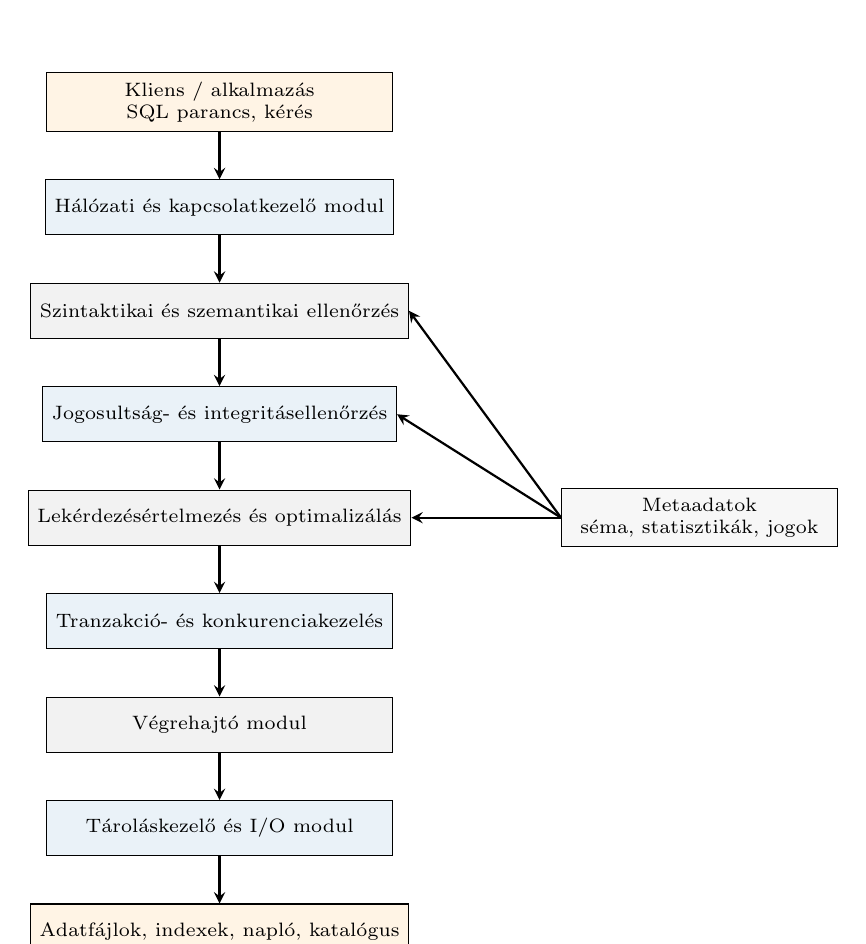
\begin{tikzpicture}[font=\scriptsize, node distance=6mm]
  \node[zvflowprocess, fill=warnbg, minimum width=44mm] (client) {Kliens / alkalmazás\\SQL parancs, kérés};
  \node[zvflowprocess, fill=lightaccent, below=of client, minimum width=44mm] (network) {Hálózati és kapcsolatkezelő modul};
  \node[zvflowprocess, fill=black!5, below=of network, minimum width=44mm] (parser) {Szintaktikai és szemantikai ellenőrzés};
  \node[zvflowprocess, fill=lightaccent, below=of parser, minimum width=44mm] (auth) {Jogosultság- és integritásellenőrzés};
  \node[zvflowprocess, fill=black!5, below=of auth, minimum width=44mm] (optimizer) {Lekérdezésértelmezés és optimalizálás};
  \node[zvflowprocess, fill=lightaccent, below=of optimizer, minimum width=44mm] (transaction) {Tranzakció- és konkurenciakezelés};
  \node[zvflowprocess, fill=black!5, below=of transaction, minimum width=44mm] (executor) {Végrehajtó modul};
  \node[zvflowprocess, fill=lightaccent, below=of executor, minimum width=44mm] (io) {Tároláskezelő és I/O modul};
  \node[zvflowprocess, fill=warnbg, below=of io, minimum width=44mm] (storage) {Adatfájlok, indexek, napló, katalógus};

  \draw[arrow] (client) -- (network);
  \draw[arrow] (network) -- (parser);
  \draw[arrow] (parser) -- (auth);
  \draw[arrow] (auth) -- (optimizer);
  \draw[arrow] (optimizer) -- (transaction);
  \draw[arrow] (transaction) -- (executor);
  \draw[arrow] (executor) -- (io);
  \draw[arrow] (io) -- (storage);

  \node[zvflowprocess, fill=black!3, right=19mm of optimizer, minimum width=35mm] (catalog) {Metaadatok\\séma, statisztikák, jogok};
  \draw[arrow] (catalog.west) -- (parser.east);
  \draw[arrow] (catalog.west) -- (auth.east);
  \draw[arrow] (catalog.west) -- (optimizer.east);
\end{tikzpicture}%
}
\caption{Egy adatkezelő parancs tipikus útja a DBMS rétegein keresztül}
\label{fig:zv21_dbms_architektura}
\end{figure}


A \textbf{lekérdezésoptimalizáló} feladata, hogy a logikai lekérdezéshez hatékony fizikai végrehajtási tervet válasszon. Például eldöntheti, hogy teljes táblabejárás, indexkeresés, hash join vagy rendezéses join legyen-e. Ehhez felhasználhatja a katalógusban tárolt metaadatokat és statisztikákat.

A \textbf{tranzakciókezelő} biztosítja, hogy az összetartozó műveletek egységként hajtódjanak végre. Ha hiba történik, a rendszer vissza tudja állítani az előző helyes állapotot. Többfelhasználós környezetben a konkurenciakezelés megakadályozza, hogy a párhuzamos műveletek hibás adatállapotot hozzanak létre.

\section{Indexek és B-fa index}

\subsection{Index fogalma és szerepe}

Az \textbf{index} olyan adatbázis-objektum, amely egy vagy több mező értékei alapján gyorsítja a rekordok megtalálását. Alapgondolata hasonlít a könyv tárgymutatójához: nem kell az egész könyvet végigolvasni, hanem a keresett kulcsszó alapján gyorsan megtaláljuk a releváns oldalt. Adatbázisban az index kulcsértékeket és az azokhoz tartozó rekord- vagy blokkmutatókat tartalmaz.

Index nélkül egy feltétel ellenőrzéséhez sokszor teljes táblabejárás kell. Indexszel a DBMS a keresett kulcstartományhoz vagy kulcsértékhez vezető úton haladhat, és kevesebb blokkot olvas. Ez különösen fontos nagy tábláknál, gyakori \code{WHERE}, \code{JOIN}, \code{ORDER BY} és \code{GROUP BY} műveleteknél.

Az indexek viszont nem ingyenesek:

\begin{itemize}
  \item tárhelyet foglalnak;
  \item beszúrás, törlés és kulcsmódosítás esetén karban kell tartani őket;
  \item túl sok index lassíthatja az adatmódosító műveleteket;
  \item az optimalizáló nem minden lekérdezésnél választ indexet, ha a teljes bejárás olcsóbb.
\end{itemize}

Ezért indexet olyan mezőkre érdemes létrehozni, amelyek gyakran szerepelnek keresési, kapcsolási vagy rendezési feltételben, és megfelelően szelektívek. Elsődleges kulcshoz sok DBMS automatikusan indexet hoz létre; idegen kulcsnál is gyakran célszerű indexet használni.

\subsection{B-fa és B+-fa jellegű index}

A \textbf{B-fa} kiegyensúlyozott keresőfa, amelyet kifejezetten háttértáras adateléréshez terveztek. Egy csomópont sok kulcsot és sok gyermekpointert tartalmazhat, ezért a fa elágazási foka nagy. Emiatt a fa magassága kicsi marad, így egy keresés kevés lemezblokk olvasásával elvégezhető.

A belső csomópontokban szereplő kulcsok útválasztóként működnek. Ha a keresett érték kisebb egy adott kulcsnál, a megfelelő bal oldali gyermek felé haladunk; ha nagyobb, a következő tartomány felé. A levelekben vagy maguk az adatmutatók, vagy B\textsuperscript{+}-fa esetén a tényleges indexbejegyzések találhatók. A B\textsuperscript{+}-fa levelei gyakran láncoltak, ami hatékony tartománykeresést tesz lehetővé.

\begin{figure}[htbp]
\centering
\resizebox{0.96\textwidth}{!}{%
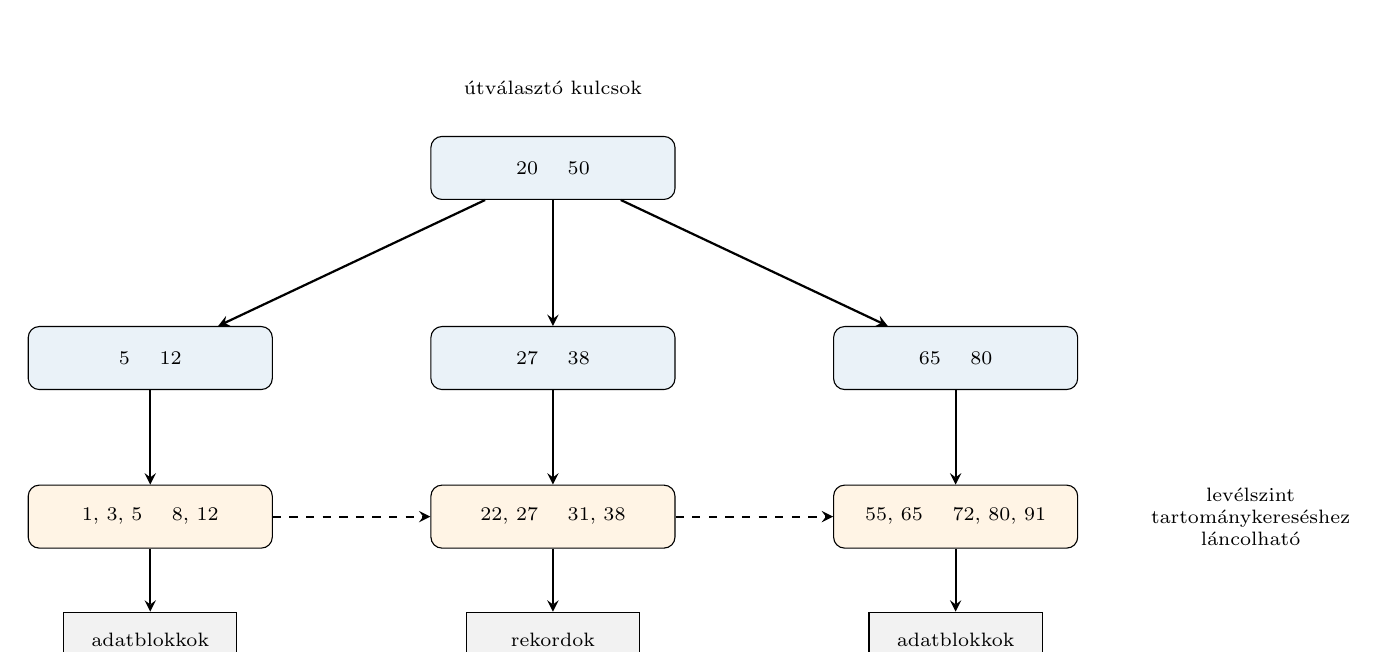
\begin{tikzpicture}[font=\scriptsize, node distance=9mm]
  \tikzset{
    bnode/.style={draw, rounded corners, fill=lightaccent, minimum width=31mm, minimum height=8mm, align=center},
    leaf/.style={draw, rounded corners, fill=warnbg, minimum width=31mm, minimum height=8mm, align=center},
    data/.style={draw, fill=black!5, minimum width=22mm, minimum height=7mm, align=center}
  }

  \node[bnode] (root) {20 \quad 50};
  \node[bnode, below left=16mm and 20mm of root] (n1) {5 \quad 12};
  \node[bnode, below=16mm of root] (n2) {27 \quad 38};
  \node[bnode, below right=16mm and 20mm of root] (n3) {65 \quad 80};

  \node[leaf, below=12mm of n1] (l1) {1, 3, 5 \quad 8, 12};
  \node[leaf, below=12mm of n2] (l2) {22, 27 \quad 31, 38};
  \node[leaf, below=12mm of n3] (l3) {55, 65 \quad 72, 80, 91};

  \node[data, below=8mm of l1] (d1) {adatblokkok};
  \node[data, below=8mm of l2] (d2) {rekordok};
  \node[data, below=8mm of l3] (d3) {adatblokkok};

  \draw[arrow] (root) -- (n1);
  \draw[arrow] (root) -- (n2);
  \draw[arrow] (root) -- (n3);
  \draw[arrow] (n1) -- (l1);
  \draw[arrow] (n2) -- (l2);
  \draw[arrow] (n3) -- (l3);
  \draw[arrow] (l1) -- (d1);
  \draw[arrow] (l2) -- (d2);
  \draw[arrow] (l3) -- (d3);

  \draw[->, >=stealth, dashed, thick] (l1.east) -- (l2.west);
  \draw[->, >=stealth, dashed, thick] (l2.east) -- (l3.west);

  \node[align=center, above=4mm of root] {útválasztó kulcsok};
  \node[align=center, right=8mm of l3] {levélszint\\tartománykereséshez\\láncolható};
\end{tikzpicture}%
}
\caption{B-fa/B\textsuperscript{+}-fa jellegű index szemléletes felépítése}
\label{fig:zv21_bfa_index}
\end{figure}


\begin{center}
\begin{tabularx}{\textwidth}{L{32mm}X}
\toprule
\textbf{Tulajdonság} & \textbf{Jelentés} \\
\midrule
Indexbejegyzés & Kulcsértékből és rekordra vagy adatblokkra mutató pointerből áll. \\
Rendezettség & A kulcsok rendezettek, ezért a keresés nem teljes táblabejárással történik. \\
B-fa csomópont & Több kulcsot és több gyermekpointert tartalmaz; egy csomópont gyakran lemezblokknak felel meg. \\
Kiegyensúlyozottság & A levelek azonos mélységben vannak, ezért a keresés útja rövid és kiszámítható. \\
Beszúrás & A megfelelő levélbe történik; telített csomópont esetén hasítás, középső kulcs felvitele és pointerigazítás szükséges. \\
Törlés & Hiányos csomópont esetén kölcsönzés vagy összevonás történhet, hogy a fa kiegyensúlyozott maradjon. \\
Költség & Tipikusan \(O(\log n)\) blokkelérés; a gyakorlatban a fa nagy elágazási foka miatt kevés szint elegendő. \\
Ár & A lekérdezések gyorsulhatnak, de az \code{INSERT}, \code{UPDATE}, \code{DELETE} műveleteknél az indexeket is frissíteni kell. \\
\bottomrule
\end{tabularx}

\end{center}

\zvpseudocode[caption={B-fa keresés vázlatos pszeudokódja}]{src/code/zv21_bfa_kereses.pseudo}

A beszúrásnál először megkeressük azt a levelet, ahová az új kulcs tartozik. Ha van hely, a kulcs bekerül rendezett pozícióba. Ha nincs hely, a csomópontot hasítani kell: a középső kulcs felkerül a szülőbe, a kulcsok egy része új testvércsomópontba kerül, és a pointerek módosulnak. Ha a szülő is megtelik, a hasítás felfelé terjedhet, akár új gyökér is létrejöhet. Ezért mondjuk, hogy a B-fa alulról felfelé és széltében növekszik.

A törlésnél ellenkező probléma jelentkezhet: egy csomópont túl kevés kulcsot tartalmaz. Ekkor a fa kölcsönzéssel vagy csomópont-összevonással állítja vissza a szükséges kihasználtságot és kiegyensúlyozottságot.

\section{Redundancia, anomáliák és funkcionális függőségek}

\subsection{Redundancia és anomáliák}

A \textbf{redundancia} ugyanannak az információs ténynek felesleges ismétlődése. Fontos, hogy nem minden azonos érték redundancia. Ha két külön embernek ugyanaz a keresztneve, az nem adatbázis-tervezési hiba. Redundanciáról akkor beszélünk, ha ugyanaz az információatom több helyen azért ismétlődik, mert rosszul választottuk meg a séma szerkezetét.

Példa rossz táblasémára:

\[
  Szerviz(rendszam, tipus, gyarto, tulajNev, tulajTelefon, datum, hibaKod, dij, szerelo)
\]

Ha ugyanaz az autó többször szerepel a táblában, akkor a \code{tipus}, \code{gyarto}, \code{tulajNev} és \code{tulajTelefon} értékek ismétlődhetnek. Ebből három klasszikus anomália származhat:

\begin{itemize}
  \item \textbf{beszúrási anomália}: új tényt csak felesleges más adatok ismétlésével lehet felvinni;
  \item \textbf{módosítási anomália}: egy tényt több rekordban kell módosítani, különben inkonzisztencia keletkezik;
  \item \textbf{törlési anomália}: egy rekord törlésével olyan információ is eltűnik, amelyet meg akartunk volna őrizni.
\end{itemize}

A normalizálás célja ezeknek az anomáliáknak a csökkentése vagy megszüntetése.

\subsection{Funkcionális függőség}

A \textbf{funkcionális függőség} azt írja le, hogy egy attribútumhalmaz értéke meghatároz egy másik attribútumhalmazt. Jelölése:

\[
  X \to Y
\]

Ez azt jelenti, hogy ha két rekordban az \(X\) attribútumhalmaz értékei megegyeznek, akkor a \(Y\) attribútumhalmaz értékeinek is meg kell egyezniük. Például ha egy rendszám egyértelműen meghatározza az autó típusát és gyártóját, akkor:

\[
  rendszam \to tipus, gyarto
\]

A redundancia egyik tipikus oka az ismétlődő értékű mezőből induló funkcionális függőség. Ha egy nagy táblában a \code{rendszam} sok sorban ismétlődik, és mindig ugyanazt a \code{tipus} és \code{gyarto} értéket hozza magával, akkor ezeket az adatokat külön relációba érdemes szervezni.

\subsection{Armstrong-axiómák és következményeik}

A funkcionális függőségek között logikai következtetéseket tehetünk. Az alapvető Armstrong-axiómák:

\begin{itemize}
  \item \textbf{reflexivitás}: ha \(Y \subseteq X\), akkor \(X \to Y\);
  \item \textbf{bővítés}: ha \(X \to Y\), akkor \(XZ \to YZ\);
  \item \textbf{tranzitivitás}: ha \(X \to Y\) és \(Y \to Z\), akkor \(X \to Z\).
\end{itemize}

Ezekből további szabályok vezethetők le. Például ha \(X \to YZ\), akkor \(X \to Y\) és \(X \to Z\) is következik. A normalizálásnál azért fontosak a függőségek, mert megmutatják, mely attribútumok tartoznak logikailag szorosan össze.

\section{Normalizálás és normálformák}

\subsection{A normalizálás szerepe}

A \textbf{normalizálás} a relációs séma olyan átalakítási folyamata, amely a redundanciát okozó függőségek megszüntetésére és a módosítási anomáliák csökkentésére törekszik. Lényege, hogy a nem megfelelően egy táblába került attribútumokat külön relációkba bontjuk, miközben a kapcsolatot kulcs--idegen kulcs viszonnyal megőrizzük.

A normalizálás nem egyszerűen „több táblára bontást” jelent. Jó normalizálásnál figyelni kell arra, hogy:

\begin{itemize}
  \item a felbontás veszteségmentes legyen;
  \item a fontos függőségek lehetőleg megőrződjenek;
  \item az anomáliák csökkenjenek;
  \item a séma továbbra is érthető és használható maradjon.
\end{itemize}

A túlzott vagy mechanikus normalizálás teljesítményproblémákat okozhat, mert sok joinra lehet szükség. Ilyenkor szabályozott denormalizálás is szóba jöhet, de ezt tudatosan, az integritási kockázatok figyelembevételével kell végezni.

\subsection{Normálformák áttekintése}

A normálformák egymásra épülő követelményeket írnak le. Minél magasabb normálformában van egy séma, annál kevesebb tipikus redundancia és anomália marad benne. A gyakorlatban a 3NF és BCNF különösen fontos vizsgaszinten.

\begin{center}
\begin{tabularx}{\textwidth}{L{18mm}L{37mm}X}
\toprule
\textbf{NF} & \textbf{Fő feltétel} & \textbf{Milyen hibát szüntet meg?} \\
\midrule
1NF & Minden mező elemi, nem listát vagy ismétlődő csoportot tartalmaz; van azonosítható rekord. & Többértékű mezők, beágyazott listák, nem relációs táblaszerkezet. \\
2NF & 1NF teljesül, és nem kulcs attribútum nem függhet csak az összetett kulcs egy részétől. & Részleges függőségek összetett kulcs esetén. \\
3NF & 2NF teljesül, és nem kulcs attribútum nem függhet más nem kulcs attribútumtól. & Tranzitív függőségek, például kulcs \(\to\) nem kulcs \(\to\) nem kulcs. \\
BCNF & Minden nemtriviális funkcionális függőség bal oldala szuperkulcs/jelölt kulcs. & A 3NF-nél erősebb követelmény; kezeli a több jelölt kulcsból adódó anomáliákat. \\
4NF & BCNF jellegű forma többértékű függőségekre: független többértékű tényeket külön kell választani. & Egymástól független többértékű kapcsolatok ismétlődései. \\
\bottomrule
\end{tabularx}

\end{center}

\subsection{1NF: első normálforma}

Egy reláció \textbf{első normálformában} van, ha minden mező értéke elemi, atomi érték. Nem tartalmazhat listát, ismétlődő csoportot vagy beágyazott táblát egy mezőben. Például a \code{hibaKodok = "2,3,5"} mező sérti az 1NF szemléletét, mert több értéket zsúfol egyetlen attribútumba.

Megoldás: a többértékű adatot külön relációba kell szervezni. Például:

\[
  Szerviz(szervizId, rendszam, datum, dij, szerelo)
\]

\[
  SzervizHiba(szervizId, hibaKod)
\]

Így minden sor egyetlen szerviz--hibakód kapcsolatot tárol.

\subsection{2NF: második normálforma}

A \textbf{második normálforma} az összetett kulcsokhoz kapcsolódik. Egy 1NF-ben lévő reláció 2NF-ben van, ha minden nem kulcs attribútum az egész kulcstól függ, és nem csak az összetett kulcs egy részétől.

Példa:

\[
  Jelentkezes(hallgatoId, targyId, hallgatoNev, targyNev, jegy)
\]

Ha a kulcs \((hallgatoId, targyId)\), akkor a \code{hallgatoNev} csak a \code{hallgatoId}-tól, a \code{targyNev} csak a \code{targyId}-tól függ. Ez részleges függőség, ezért sérti a 2NF-et. Helyesebb bontás:

\[
  Hallgato(hallgatoId, hallgatoNev)
\]

\[
  Targy(targyId, targyNev)
\]

\[
  Jelentkezes(hallgatoId, targyId, jegy)
\]

\subsection{3NF: harmadik normálforma}

A \textbf{harmadik normálforma} a tranzitív függőségek megszüntetésére irányul. Egy reláció 3NF-ben van, ha 2NF-ben van, és nem kulcs attribútum nem függ más nem kulcs attribútumtól.

Példa:

\[
  Auto(rendszam, tipus, gyartoNev, gyartoOrszag)
\]

Ha \code{rendszam} a kulcs, és \code{gyartoNev \to gyartoOrszag}, akkor a \code{gyartoOrszag} tranzitívan függ a rendszámtól:

\[
  rendszam \to gyartoNev \to gyartoOrszag
\]

Ezt külön táblába érdemes szervezni:

\[
  Auto(rendszam, tipus, gyartoNev)
\]

\[
  Gyarto(gyartoNev, gyartoOrszag)
\]

\subsection{BCNF: Boyce--Codd normálforma}

A \textbf{BCNF} erősebb követelmény, mint a 3NF. Egy reláció BCNF-ben van, ha minden nemtriviális funkcionális függőség \(X \to Y\) esetén \(X\) szuperkulcs. Másként: csak kulcs jellegű attribútumhalmaz határozhat meg más attribútumot.

Ez különösen akkor fontos, ha több jelölt kulcs van, vagy a 3NF még megengedne olyan függőséget, amely anomáliát okozhat. Ha egy reláció nem BCNF, akkor a sértő függőség mentén felbontjuk.

\zvpseudocode[caption={BCNF-dekompozíció vázlatos algoritmusa}]{src/code/zv21_bcnf_dekompozicio.pseudo}

A BCNF-re bontás általában csökkenti a redundanciát, de nem mindig őriz meg minden funkcionális függőséget egyszerűen ellenőrizhető formában. Ezért a gyakorlatban néha választani kell a szigorúbb normalizálás és a függőségmegőrzés között.

\subsection{4NF röviden}

A \textbf{negyedik normálforma} többértékű függőségekhez kapcsolódik. Akkor válik fontossá, ha egy egyedhez több, egymástól független többértékű tulajdonság tartozik. Például egy oktató több nyelven beszélhet és több tárgyat taníthat, de a nyelvek és tárgyak egymástól függetlenek. Ha ezeket egyetlen táblában tároljuk, mesterséges kombinációk és ismétlődések keletkezhetnek.

Ilyenkor külön relációk használata helyesebb:

\[
  OktatoNyelv(oktatoId, nyelv)
\]

\[
  OktatoTargy(oktatoId, targyId)
\]

Vizsgán általában elég jelezni, hogy a 4NF a többértékű függőségek okozta redundanciát kezeli, míg az 1NF--BCNF főleg funkcionális függőségekre épül.

\section{Dekompozíció célja és szabályai}

\subsection{Dekompozíció fogalma}

A \textbf{dekompozíció} egy relációséma felbontása több kisebb relációsémára. Például:

\[
  Auto(rendszam, tipus, gyarto)
\]

felbontható erre:

\[
  Auto(rendszam, tipus)
\]

\[
  TipusGyarto(tipus, gyarto)
\]

ha a \(tipus \to gyarto\) függőség ezt indokolja. A cél nem az információ törlése, hanem az, hogy a nem egy táblába tartozó függőségeket külön relációkban tároljuk.

Dekompozíció után az eredeti kapcsolatok általában elsődleges kulcsokkal és idegen kulcsokkal jelennek meg. A felbontás akkor jó, ha az eredeti adatállapot visszaállítható, és nem keletkeznek hamis kombinációk.

\subsection{Veszteségmentesség és függőségmegőrzés}

A két legfontosabb elvárás:

\begin{itemize}
  \item \textbf{veszteségmentes felbontás}: a résztáblák joinjából visszakapható az eredeti reláció;
  \item \textbf{függőségmegőrzés}: az eredeti függőségek ellenőrizhetők a részsémákon is.
\end{itemize}

Ha a felbontás nem veszteségmentes, akkor adatvesztés vagy hamis rekordok keletkezhetnek. Ha nem függőségmegőrző, akkor bizonyos megkötések ellenőrzéséhez össze kell joinolni a táblákat, ami bonyolultabb és drágább.

\begin{center}
\begin{tabularx}{\textwidth}{L{35mm}X}
\toprule
\textbf{Elvárás vagy tétel} & \textbf{Lényege} \\
\midrule
Veszteségmentes felbontás & A felbontott relációk természetes joinjából visszaállítható az eredeti reláció, vagyis nem keletkezik hamis rekord és nem vész el információ. \\
Függőségmegőrzés & Az eredeti funkcionális függőségek ellenőrizhetők a felbontott sémákon is anélkül, hogy mindig össze kellene joinolni őket. \\
Heath-tétel & Ha \(R(A,B,C)\) relációban \(A \to B\) teljesül, akkor az \(R_1(A,B)\) és \(R_2(A,C)\) felbontás veszteségmentes. \\
Rissanen-tétel & Egy felbontás akkor tekinthető függetlennek, ha a függőségrendszer előállítható a részsémák függőségeiből, és a közös attribútum megfelelő kulcsszerepet tölt be valamelyik részsémában. \\
Normalizálási lépés & A redundanciát okozó függőség bal oldalát és a tőle függő mezőket külön relációba tesszük, majd PK--FK kapcsolattal kötjük össze a részeket. \\
Kompromisszum & A normalizálás csökkenti az anomáliákat, de több joinhoz vezethet; teljesítmény miatt néha szabályozott denormalizálás indokolt. \\
\bottomrule
\end{tabularx}

\end{center}

\subsection{Heath-tétel}

A \textbf{Heath-tétel} egy klasszikus veszteségmentes felbontási eredmény. Ha adott egy:

\[
  R(A,B,C)
\]

reláció, és teljesül:

\[
  A \to B,
\]

akkor az

\[
  R_1(A,B) \quad \text{és} \quad R_2(A,C)
\]

felbontás veszteségmentes. Intuitívan azért, mert \(A\) meghatározza \(B\)-t, ezért az \(A\) szerinti visszakapcsolás nem hoz létre hamis \(B\)-értékeket. Ez a normalizálás egyik alapgondolata: a kulcs jellegű meghatározó mező és a tőle függő attribútumok kerüljenek külön relációba.

\subsection{Rissanen-tétel és független felbontás}

A \textbf{Rissanen-tétel} a független felbontás feltételeit fogalmazza meg. Egyszerű vizsgaszinten elég úgy megjegyezni, hogy a felbontás akkor jó erősebb értelemben, ha:

\begin{itemize}
  \item az eredeti függőségrendszer előállítható a részsémák függőségeiből;
  \item a közös attribútumhalmaz valamelyik részsémában kulcsszerepet tölt be.
\end{itemize}

Ez biztosítja, hogy a résztáblák ne mesterségesen egymástól függő darabok legyenek, hanem valóban önálló jelentésű relációk.

\section{Összefüggő normalizálási példa}

\subsection{Kiinduló séma}

Legyen a kiinduló táblánk:

\[
  Szerviz(rendszam, tipus, gyarto, tulajNev, tulajTelefon, datum, hibaKod, dij, szerelo)
\]

Tegyük fel a következő függőségeket:

\begin{itemize}
  \item \(rendszam \to tipus, tulajNev\);
  \item \(tipus \to gyarto\);
  \item \(tulajNev \to tulajTelefon\) az egyszerűsített példában;
  \item \(hibaKod \to dij\);
  \item egy szervizeseményt a \((rendszam, datum, hibaKod)\) azonosít.
\end{itemize}

A séma sok redundanciát tartalmaz. Egy autó típusa és tulajdonosa minden szervizalkalomnál ismétlődhet, a típus gyártója is ismétlődhet, a hibakódhoz tartozó díj is több sorban megjelenhet.

\subsection{Felbontás}

Egy lehetséges normalizáltabb felbontás:

\[
  Auto(rendszam, tipus, tulajNev)
\]

\[
  Tipus(tipus, gyarto)
\]

\[
  Tulajdonos(tulajNev, tulajTelefon)
\]

\[
  Hiba(hibaKod, dij)
\]

\[
  Szerviz(rendszam, datum, hibaKod, szerelo)
\]

A redundáns információk külön táblákba kerültek. Ha egy tulajdonos telefonszáma változik, elég a \code{Tulajdonos} táblában módosítani. Ha egy hibakód díja változik, elég a \code{Hiba} táblát frissíteni. Az eseményeket a \code{Szerviz} tábla köti össze az autóval és a hibakóddal.

\subsection{Értelmezés}

Ez a felbontás csökkenti a módosítási anomáliákat és átláthatóbbá teszi az adatmodellt. A fizikai teljesítmény ugyanakkor függ a lekérdezésektől. Ha gyakran kell minden adatot együtt megjeleníteni, több joinra lesz szükség, ezért az idegen kulcsokra és gyakori keresési mezőkre indexeket érdemes létrehozni.

Itt látszik a tétel két része közötti kapcsolat: a \textbf{logikai tervezés} normalizálással alakítja ki a helyes sémát, a \textbf{fizikai tervezés} pedig indexekkel, fájlszervezéssel és tárolási döntésekkel teszi hatékonnyá a használatot.

\section{Gyakori vizsgahibák és összefoglalás}

\subsection{Gyakori félreértések}

\begin{itemize}
  \item \textbf{Adatbázis és DBMS összekeverése.} Az adatbázis a tárolt adatrendszer, a DBMS az ezt kezelő szoftverrendszer.
  \item \textbf{Fájlkezelés és adatbáziskezelés teljes azonosítása.} A DBMS fájlokat használhat fizikailag, de logikailag sémát, tranzakciókat, jogosultságokat és lekérdező nyelvet is ad.
  \item \textbf{Index túlértékelése.} Az index gyorsíthatja a keresést, de tárhelyet foglal és lassíthatja a módosításokat.
  \item \textbf{B-fa és bináris keresőfa összekeverése.} A B-fa többkulcsos, nagy elágazási fokú, kiegyensúlyozott fa, amely háttértáras blokkelérésre alkalmas.
  \item \textbf{Redundancia félreértése.} Nem minden ismétlődő érték redundancia; redundancia az ismétlődő információs tény.
  \item \textbf{1NF kihagyása.} Listák és ismétlődő csoportok mezőben tárolása sérti a relációs szemléletet.
  \item \textbf{2NF és 3NF összekeverése.} A 2NF részleges függőséget kezel összetett kulcsnál, a 3NF tranzitív függőséget nem kulcs mezők között.
  \item \textbf{BCNF túl rövid definíciója.} A lényege: minden nemtriviális funkcionális függőség bal oldala legyen szuperkulcs.
  \item \textbf{Dekompozíció veszteségmentességének elhanyagolása.} Nem elég táblákat szétszedni; az eredeti információt vissza kell tudni állítani.
  \item \textbf{Normalizálás és teljesítmény viszonyának elhallgatása.} A normalizálás logikai tisztaságot ad, de fizikai szinten indexekre és néha denormalizálásra is szükség lehet.
\end{itemize}

\subsection{Rövid vizsgaválasz-minta}

\begin{summarybox}
Az adatkezelés az adatok létrehozását, tárolását, lekérdezését, módosítását, törlését és védelmét jelenti. Fájlalapú megoldásnál az alkalmazás közvetlenül fájlokat kezel, ismeri a rekordok szerkezetét, és maga valósítja meg a keresést, módosítást, védelmet és konkurenciakezelést. Ez egyszerű esetekben elég lehet, de nagyobb rendszereknél rugalmatlan, nehezen védhető és lassú lehet. A DBMS olyan adatbázis-kezelő rendszer, amely sémával, metaadatokkal, lekérdező nyelvvel, indexekkel, jogosultságkezeléssel, tranzakciókezeléssel és optimalizálással biztosítja az adatok hatékony kezelését. A fájlszervezési módszerek közé tartozik a heap, szekvenciális, index-szekvenciális, indexelt, hash, klaszterezett és particionált tárolás. Az index kulcsérték--pointer párokkal gyorsítja a keresést; gyakori megvalósítása a kiegyensúlyozott, többkulcsos B-fa vagy B\textsuperscript{+}-fa, amely kevés blokkeléréssel támogatja a pont- és tartománykeresést. A normalizálás a redundanciát okozó funkcionális függőségek megszüntetésére irányuló sémaátalakítás. Az 1NF elemi mezőket vár el, a 2NF megszünteti az összetett kulcs részétől való függést, a 3NF megszünteti a nem kulcs mezőből induló tranzitív függést, a BCNF pedig azt követeli meg, hogy minden nemtriviális függőség bal oldala szuperkulcs legyen. A dekompozíció jó esetben veszteségmentes és lehetőleg függőségmegőrző; fontos eredmény a Heath-tétel, amely funkcionális függőség alapján ad veszteségmentes felbontást.
\end{summarybox}

\end{document}
